\section{Irradiation at the Rhode Island Neutron Irradiation Facility}
\label{sec:irradiation}

\subsection{Rhode Island Nuclear Reactor}
\label{subsec:RINSC}
The Rhode Island Nuclear Science Center (RINSC) is a \SI{2}{\mega\watt}, light-water cooled, pool-type reactor in Narragansett, Rhode Island, USA.
Its core consists of fuel assemblies reflected with a combination of graphite and beryllium.
The fuel is plate type U$_3$Si$_2$ cladded with aluminum enriched to less than 20$~\%$ Uranium-235.
At RINSC, there are six different methods to irradiate materials, but only one of these, the 8'' beamport, will be discussed in this paper.
Namely, it is the only sample delivery system large enough to accept full-sized HGCAL silicon sensor wafers and therefore has been revived for this project after its last usage 30 years ago.\newline
A sketch and a photo of the inside of this beamport are shown in \ref{fig:Beamport_Schematic}a and b.
\begin{figure}[!hbt]
  \begin{center}
    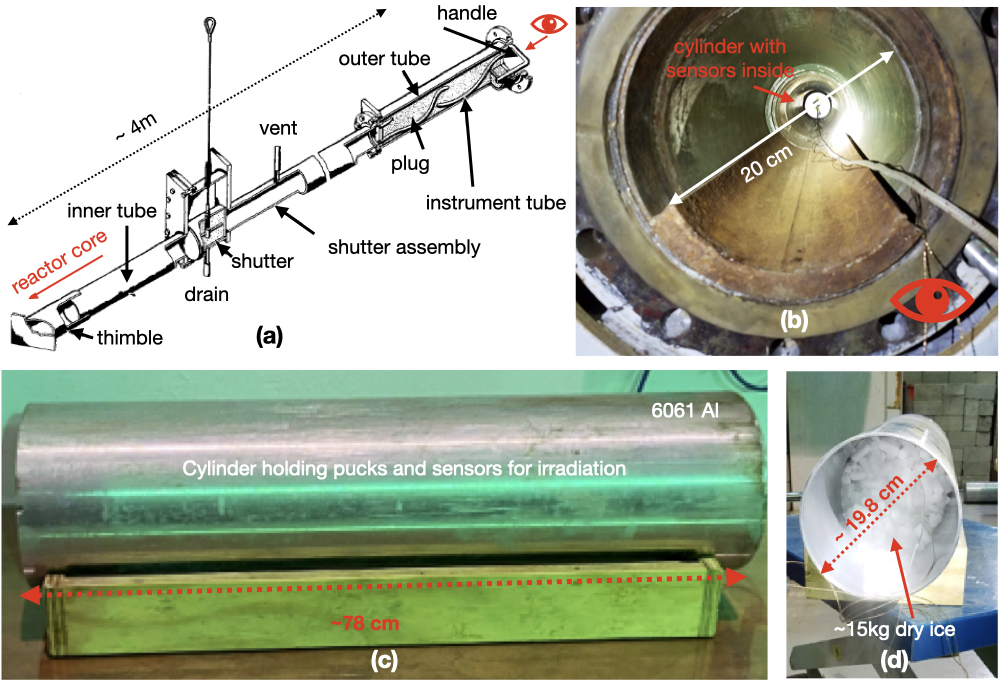
\includegraphics[width=0.99\textwidth]{figures/figures_edited_001.jpeg}
    \caption{(a) Schematic of one of the beamport sample delivery systems at the RINSC Facility.
    (b) The view down into the beamport used for these irradiation studies.
    (c) The sample delivery cylinder that contains the sensor-holding hockey pucks and (d) dry ice for cooling of the silicon sensors during and after irradiation.
    }
    \label{fig:Beamport_Schematic}
  \end{center}
\end{figure}
It measures about \SI{4}{\metre} from the opening to the termination near to the reactor core, and it can accommodate samples with diameters of up to \SI{20}{\centi\metre} and a depth of about \SI{90}{\centi\metre}.
A shutter assembly sits \SI{3}{\metre} from the opening of the beamport, which must be raised to allow for the insertion of the experimental setup and closed prior to the start of the reactor.
A \SI{85}{\centi\metre}-long lead plug serves as a radiation shield that has to be inserted into the opening of the beamport prior to the start of irradiation.

\subsection{Irradiation of HGCAL silicon sensor prototypes}
\label{subsec:irradiation}
Given the constraints of the beamport system at RINSC, a dedicated sample delivery method was developed for irradiation HGCAL silicon wafers.
This new sample delivery allows for:
\begin{itemize}
  \item Positioning sensors as close to the reactor core as possible,
  \item protecting them from physical damage during the loading, irradiation, and unloading,
  \item keeping the irradiated sensors at cold temperatures during the after the irradiation,
  \item and monitoring the temperature of the samples inside the reactor.
\end{itemize}
Two compatible pieces of hardware were developed for the irradiation of these silicon sensors: a sensor container, referred to as a hockey puck, and a sample delivery cylinder (see~\ref{fig:Beamport_Schematic}c). 
The former is used to protect, orient, and store the sensors during irradiation while the latter is used to protect and locate the hockey puck inside the beamport.\newline
The cylinder is made from 6061 aluminum, has an outer diameter of \SI{19.8}{\centi\metre} fitting into the beamport, and the inner diameter of the cylinder \SI{19.1}{\centi\metre} allowing for smooth insertion and removal of the hockey pucks.
The cylinder has a welded cap on the end that faces the reactor core and a removable cap with threaded holes for 8 to 32 countersunk flat head machine screws that are flush with the outer wall of the cylinder. 
Both the welded cap and removable cap have vent holes to allow for air to flow into and out of the cylinder.
An eye bolt is screwed into the removable cap to facilitate removing the cylinder from the beamport after irradiations.\newline
The hockey pucks have been made from a variety of different materials including oak, acrylic, and PEEK, see~\ref{fig:Pucks_Arrayed}a. 
\begin{figure}[!hbt]
  \begin{center}
    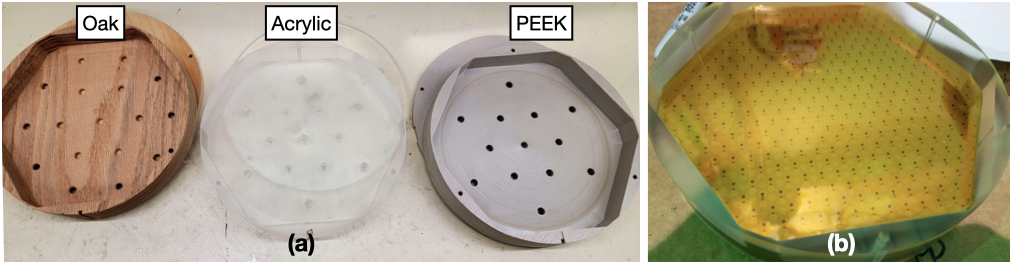
\includegraphics[width=0.99\textwidth]{figures/figures_edited_002.jpeg}
    \caption{(a) Sample containers ('hockey pucks') holding HGCAL silicon sensors for neutron irradiation at RINSC. 
    The deployed materials were wood (oak), acrylic, and PEEK.
    (b) An 8'' high-density HGCAL prototype silicon sensor inside an acrylic puck closed with a Kapton\texttrademark$~$foil.}
    \label{fig:Pucks_Arrayed}
  \end{center}
\end{figure}
The puck base has an outer diameter of \SI{18.6}{\milli\metre} that allows for a smooth fit inside the cylinder. 
Its interior of the puck is milled out in the profile of the silicon sensors with an additional clearance of \SI{1}{\milli\metre}. 
With these constraints the thinnest sections of the wall of the puck are slightly over \SI{1}{\milli\metre} thick which provides a difficult machining challenge.
The puck has a lid, made from the same material as the base, that matches the outer diameter of the base and provides a way to close the puck during handling.
Matching through holes in the base and lid allow for using nylon threaded rods and nuts to fasten the puck together. \newline
Kapton\texttrademark$~$foils were used to separate sensors in a stack such that no sensors are in direct contact with any rough surfaces (cf.~\ref{fig:Pucks_Arrayed}b).
In addition, antistatic foam was used for covering the top and bottom of sensor-Kapton\texttrademark stack serving as a cushion  against the walls inside the puck.
Sensors were irradiated in batches of four, which required ten layers of Kapton\texttrademark$~$foils and three to four layers of antistatic foam. 
After preparation of the puck it was inserted into the delivery cylinder.
In general, sensors should ideally be kept at low temperatures during the irradiation in order to limit unwanted annealing.
For this purpose, the rest of the cylinder was filled with 15-\SI{18}{\kilo\gram} of dry ice.
However, it was found empirically that most of the dry ice is eventually consumed during irradiation.
Therefore, PT1000 resistance temperature detectors (RTD) were inserted into the puck, at the front or back face, to record the temperature throughout the irradiation for assessment of the expected sensor annealing during irradiation.
Before the cylinder was closed, the RTD wires were routed through the vent holes in the removable cap, and were connected to a dedicated temperature readout system outside the beamport.\newline 
Once the cylinder had been fully packed it was loaded onto a sled and inserted into the opening of the beamport.
It was then pushed all the way inside, the shutter was lowered, the lead plug was inserted into the opening of the beamport, and the setup was ready for irradiation.\newline
A representative temperature recording during irradiation is shown in~\ref{fig:Round_10_Temperature_Profile}.
\begin{figure}[!hbt]
  \begin{center}
    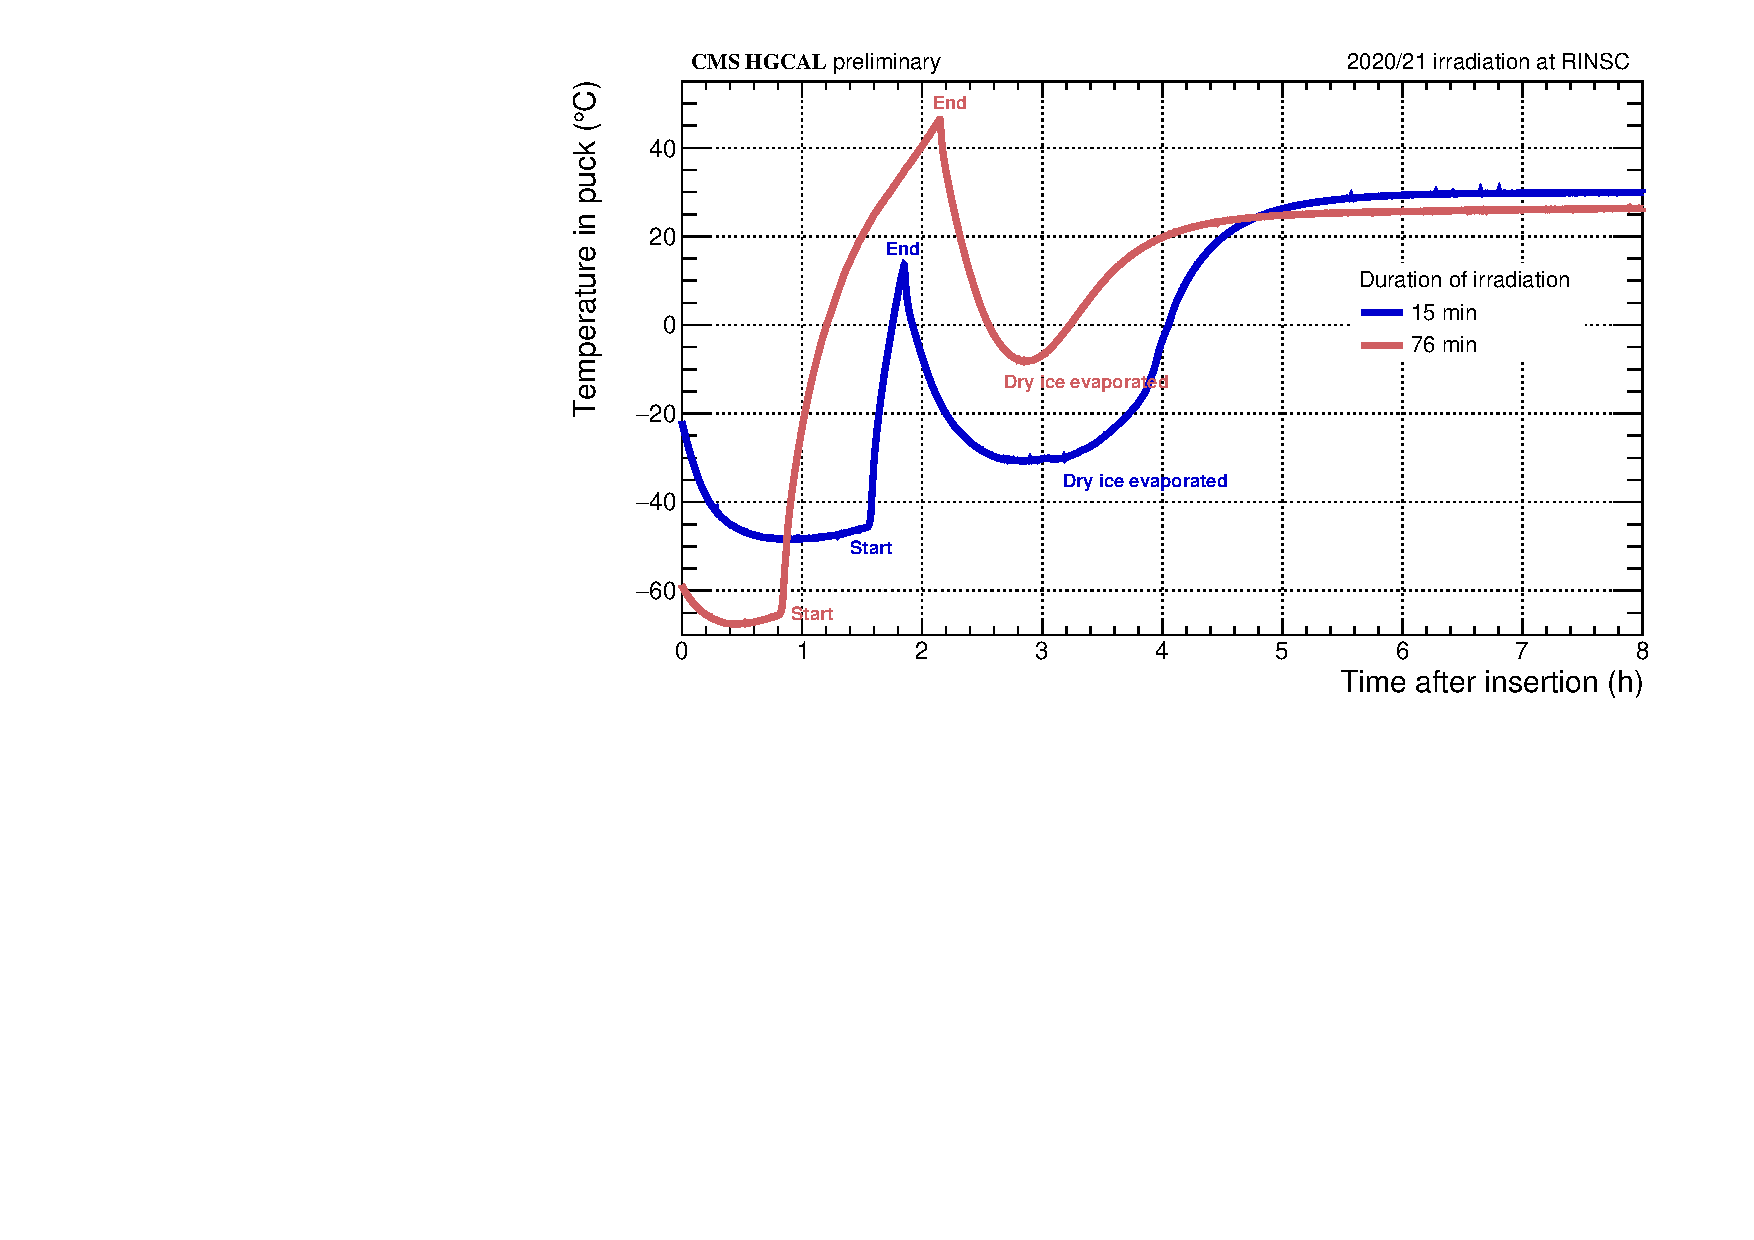
\includegraphics[width=0.69\textwidth]{plots/RINSC_temp/RINSC_temp.pdf}
    \caption{Representative temperature recordings during two of the RINSC irradiation rounds of HGCAL prototype silicon sensors. 
    The time when the irradiation was started and when it ended is indicated.
    The increase of the temperature towards its plateau coincides with the evaporation of the dry ice inside the delivery cylinder.
    }
    \label{fig:Round_10_Temperature_Profile}
  \end{center}
\end{figure}
The start up of the reactor takes about 50-\SI{100}{\minute}. 
Once the reactor operated at full capacities, the recorded temperature increased significantly and continued to increase throughout the duration of the irradiation.
As a result, the annealing of the silicon sensors inside the beam port was in fact not negligible.
It varied for the neutron-irradiated sensors between a few minutes to a few hundred minutes equivalent to \SI{60}{\celsius}.
Only after shutdown of the reactor, the temperature decreased again.
After \SI{24}{\hour} in the beamport after irradiation, the cylinder's radioactive levels have decayed sufficiently such that it could safely be transferred into a storage freezer.

\subsection{Fluence Assessment}
In addition to the sensors, mechanical packing material, and temperature sensors, each puck contained a number of reference objects for measuring the fluence achieved during an irradiation round. 
Two different objects were found appropriate for measuring the fluences during this campaign: Reference silicon diodes from the D0 experiment, and ultrapure iron foils. 
The diodes were included inside the puck as close to the sensors as possible by encasing them in small plastic bags and taping them to the inside faces of the puck. 
By contrast, the iron foils were attached to the exterior of the cylinder for ease of removal and rapid counting. \newline
After irradiation, gamma spectra of the iron foils are measured at RINSC and the fluence was derived from this data.
In addition, CV and IV measurements of the irradiated diodes were performed at Brown university to assess the depletion voltage, the associated dark current and ultimately the fluence assuming the literature value for the current-related leakage current rate.\newline
%It was found empirically that the usage of commercially-available pin diodes saturated already at low fluences (below 4E14) and thus were not found to be particularly useful. 
The reference silicon diodes are most useful up for the lower to medium range of the targeted fluences,  where their depletion voltage was well within the measurement range ($<\SI{1000}{\volt}$).
For higher fluences, full depletion of the silicon diodes could not be reached, and the gamma ray spectra derived from the iron foils are considered more reliable.
\ref{table:irrads} in~\ref{appendix:irrad_rounds} shows the estimated actual fluences from those reference structures.\newline
In order to improve the reliability of those reference fluence measurements, future irradiation of HGCAL silicon wafers at RINSC will include iron foils inside the puck as well as additional test structures of HGCAL silicon sensors.